% Options for packages loaded elsewhere
\PassOptionsToPackage{unicode}{hyperref}
\PassOptionsToPackage{hyphens}{url}
\documentclass[
]{antposter}
\usepackage{xcolor}
\usepackage{amsmath,amssymb}
\setcounter{secnumdepth}{-\maxdimen} % remove section numbering
\usepackage{iftex}
\ifPDFTeX
  \usepackage[T1]{fontenc}
  \usepackage[utf8]{inputenc}
  \usepackage{textcomp} % provide euro and other symbols
\else % if luatex or xetex
  \usepackage{unicode-math} % this also loads fontspec
  \defaultfontfeatures{Scale=MatchLowercase}
  \defaultfontfeatures[\rmfamily]{Ligatures=TeX,Scale=1}
\fi
\usepackage{lmodern}
\ifPDFTeX\else
  % xetex/luatex font selection
\fi
% Use upquote if available, for straight quotes in verbatim environments
\IfFileExists{upquote.sty}{\usepackage{upquote}}{}
\IfFileExists{microtype.sty}{% use microtype if available
  \usepackage[]{microtype}
  \UseMicrotypeSet[protrusion]{basicmath} % disable protrusion for tt fonts
}{}
\makeatletter
\@ifundefined{KOMAClassName}{% if non-KOMA class
  \IfFileExists{parskip.sty}{%
    \usepackage{parskip}
  }{% else
    \setlength{\parindent}{0pt}
    \setlength{\parskip}{6pt plus 2pt minus 1pt}}
}{% if KOMA class
  \KOMAoptions{parskip=half}}
\makeatother
\setlength{\emergencystretch}{3em} % prevent overfull lines
\providecommand{\tightlist}{%
  \setlength{\itemsep}{0pt}\setlength{\parskip}{0pt}}
\qrdata{www.instagram.com/agireperilfuturo}
\abstract{ \textbf{Notizie dell'Ultimo Momento:}\ \begin{itemize} \item \textbf{Emissioni in aumento}: Le emissioni globali di CO2 hanno raggiunto un nuovo massimo nel 2024. \item \textbf{Rinnovabili in crescita}: Capacità di energia solare ed eolica aumentata rispetto al 2023. \item \textbf{Iniziative urbane}: Nuove piste ciclabili e zone a traffico limitato in molte città europee. \end{itemize}
\begin{center}\rule{0.5\linewidth}{0.5pt}\end{center} \begin{center}\end{center}
\textbf{Iniziative per Giovani sul Territorio:}\ \begin{itemize} \item \textbf{Green Camp Week} (25-30 marzo 2025, Milano): Workshop su energia rinnovabile e agricoltura urbana. \item \textbf{Eco-Design Challenge} (10 aprile 2025, Torino): Concorso per progettare prodotti sostenibili. \item \textbf{Pianta il Futuro} (22 aprile 2025, Roma): Giornata dedicata alla piantumazione di alberi urbani. \end{itemize}
\begin{center}\rule{0.5\linewidth}{0.5pt}\end{center} \begin{center}\end{center}
\centerline{ 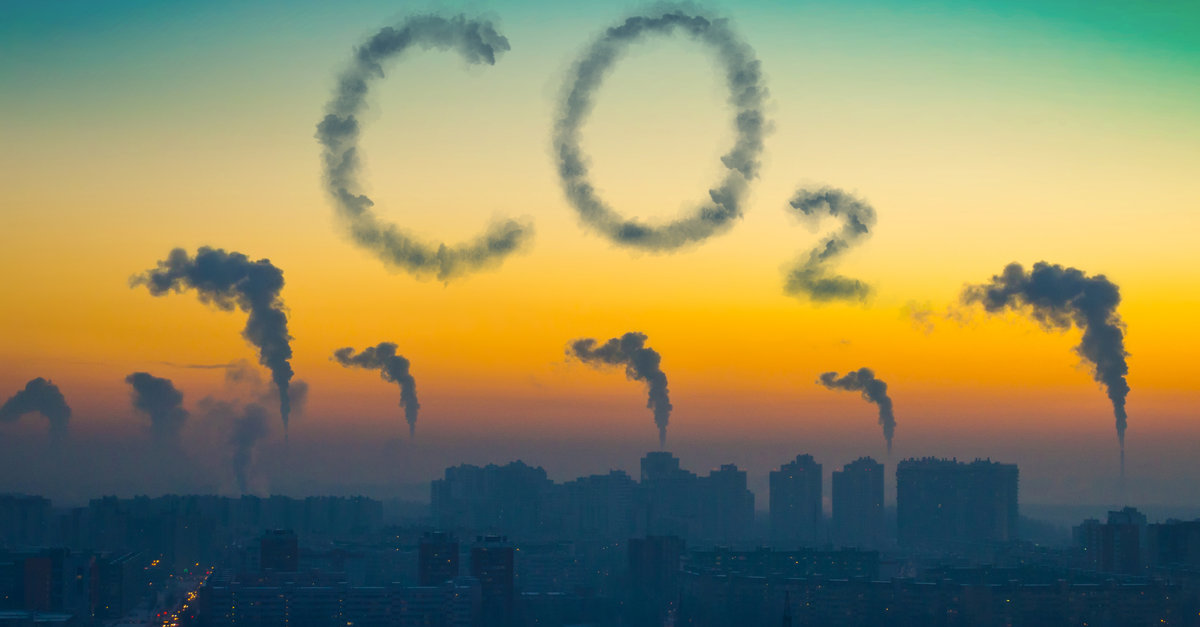
\includegraphics[height=5.5cm]{./foto/co2.jpg}   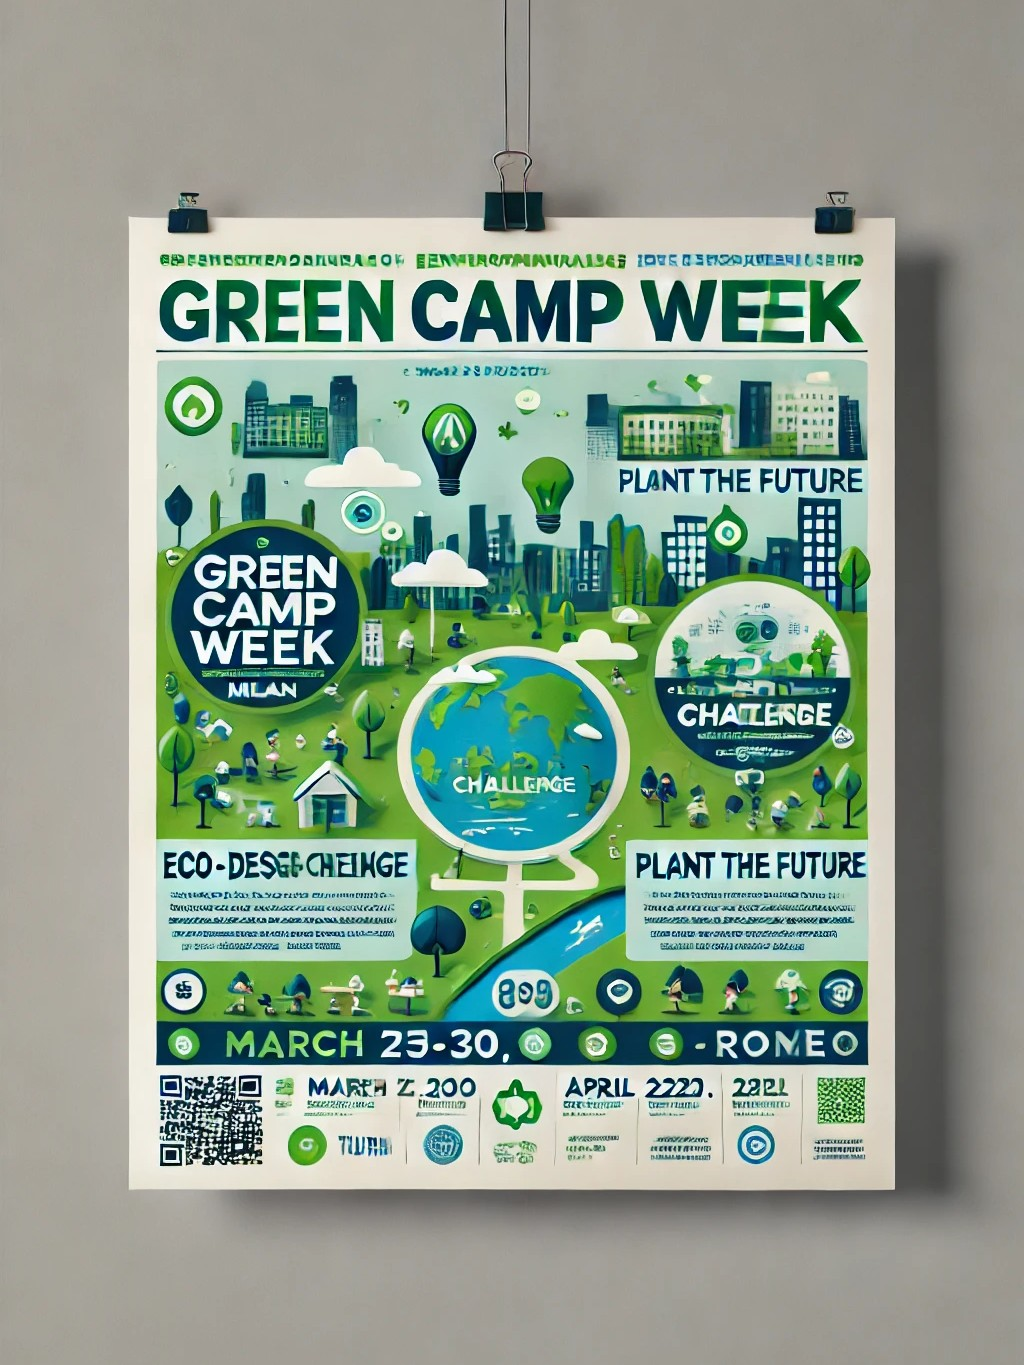
\includegraphics[height=5.5cm]{./foto/poster.jpg}} }
\usepackage{bookmark}
\IfFileExists{xurl.sty}{\usepackage{xurl}}{} % add URL line breaks if available
\urlstyle{same}
\hypersetup{
  pdftitle={Agire per il Futuro: Guida alla Sostenibilità},
  pdfauthor={Salvatore Torrisi},
  hidelinks,
  pdfcreator={LaTeX via pandoc}}

\title{Agire per il Futuro: Guida alla Sostenibilità}
\author{Salvatore Torrisi}
\date{2025-01-14}

\begin{document}
\maketitle

\subsection{Introduzione}\label{introduzione}

Il cambiamento climatico è una delle sfide più urgenti e significative
del nostro tempo. Gli impatti di questo fenomeno globale si manifestano
attraverso eventi meteorologici estremi, l'innalzamento del livello del
mare, e la perdita di biodiversità. Tuttavia, ognuno di noi ha il potere
di fare la differenza attraverso le proprie scelte quotidiane.

Questo prodotto editoriale è pensato per aiutarti a comprendere meglio
il cambiamento climatico e fornirti strumenti pratici per ridurre il tuo
impatto ambientale. Perché ogni piccolo gesto conta!

\begin{center}\rule{0.5\linewidth}{0.5pt}\end{center}

\subsection{Dati Scientifici}\label{dati-scientifici}

\subsubsection{Che cos'è il cambiamento
climatico?}\label{che-cosuxe8-il-cambiamento-climatico}

Il cambiamento climatico si riferisce a variazioni a lungo termine delle
temperature e dei modelli climatici globali. Questi cambiamenti sono
spesso attribuiti alle attività umane, in particolare all'emissione di
gas serra come anidride carbonica (CO2), metano (CH4) e protossido di
azoto (N2O).

\subsubsection{Alcuni dati chiave}\label{alcuni-dati-chiave}

\begin{itemize}
\tightlist
\item
  \textbf{+1,1°C}: La temperatura media globale è aumentata di circa
  1,1°C rispetto all'epoca preindustriale.
\item
  \textbf{30\%}: Circa il 30\% delle emissioni di gas serra proviene dal
  sistema alimentare globale.
\item
  \textbf{11 anni}: Gli ultimi 11 anni sono stati i più caldi mai
  registrati nella storia moderna.
\item
  \textbf{1 milione di specie a rischio}: La perdita di habitat e il
  riscaldamento globale mettono a rischio un milione di specie animali e
  vegetali.
\end{itemize}

\subsubsection{Perché è importante agire
ora?}\label{perchuxe9-uxe8-importante-agire-ora}

Gli scienziati sottolineano che abbiamo poco tempo per limitare
l'aumento della temperatura globale a 1,5°C, soglia oltre la quale gli
impatti del cambiamento climatico diventeranno catastrofici.

\begin{center}\rule{0.5\linewidth}{0.5pt}\end{center}

\subsection{Esempi di Azioni
Sostenibili}\label{esempi-di-azioni-sostenibili}

\subsubsection{Riduci gli sprechi
alimentari}\label{riduci-gli-sprechi-alimentari}

Gli sprechi alimentari rappresentano una delle principali fonti di
emissioni di gas serra. Ogni anno, circa un terzo del cibo prodotto a
livello globale viene sprecato. Puoi contribuire a ridurre questi
sprechi con semplici azioni:

\begin{itemize}
\tightlist
\item
  \textbf{Compra consapevolmente}: Pianifica i tuoi pasti e compra solo
  ciò di cui hai bisogno.
\item
  \textbf{Conserva correttamente}: Usa contenitori ermetici e conserva
  gli alimenti in luoghi adeguati per prolungarne la durata.
\item
  \textbf{Riutilizza gli avanzi}: Trasforma gli avanzi in nuovi piatti
  creativi invece di buttarli via.
\end{itemize}

\subsubsection{Scegli una mobilità
sostenibile}\label{scegli-una-mobilituxe0-sostenibile}

Il settore dei trasporti è responsabile di circa il 24\% delle emissioni
globali di CO2. Per ridurre il tuo impatto:

\begin{itemize}
\tightlist
\item
  Usa i mezzi pubblici o condividi l'auto.
\item
  Spostati a piedi o in bicicletta per brevi distanze.
\item
  Considera l'acquisto di un'auto elettrica o ibrida.
\end{itemize}

\subsubsection{Riduci il consumo di
plastica}\label{riduci-il-consumo-di-plastica}

La plastica monouso contribuisce all'inquinamento degli oceani e alla
distruzione degli ecosistemi. Alcuni consigli utili:

\begin{itemize}
\tightlist
\item
  Porta con te una borraccia riutilizzabile.
\item
  Usa borse di tela per la spesa.
\item
  Evita prodotti con imballaggi eccessivi.
\end{itemize}

\subsubsection{Adotta una dieta più
sostenibile}\label{adotta-una-dieta-piuxf9-sostenibile}

La produzione alimentare, in particolare quella di carne e latticini, ha
un grande impatto sull'ambiente. Ecco come puoi fare la differenza:

\begin{itemize}
\tightlist
\item
  Riduci il consumo di carne, specialmente quella rossa.
\item
  Scegli prodotti locali e di stagione.
\item
  Prova nuove ricette a base vegetale.
\end{itemize}

\begin{center}\rule{0.5\linewidth}{0.5pt}\end{center}

\subsection{Call-to-Action}\label{call-to-action}

Ora che hai appreso come puoi contribuire alla lotta contro il
cambiamento climatico, è il momento di agire! Condividi queste
informazioni con i tuoi amici e la tua famiglia. Ecco alcune idee per
cominciare:

\begin{itemize}
\tightlist
\item
  \textbf{Partecipa a iniziative locali}: Partecipa a eventi di pulizia
  ambientale o progetti di riforestazione.
\item
  \textbf{Condividi sui social}: Usa i tuoi canali social per
  sensibilizzare altre persone.
\item
  \textbf{Firma petizioni}: Sostieni leggi e politiche che promuovono la
  sostenibilità.
\end{itemize}

Ricorda: ogni gesto conta, e insieme possiamo fare la differenza.

\begin{center}\rule{0.5\linewidth}{0.5pt}\end{center}

\end{document}
